\scanpage{88}
\mspage{84}
% archive sheet number: 87

\uline{Corollaire \unsure{5|3}} Soient $(E,\leq,\mathrel{|{\circ}|})$ un \unsure{disjoncteur} \unsure{préordonné}, et soit $E'$ une partie de $E$ qui est ``dense'' dans le sens suivant
\[
\forall x,y\in E,\quad\deleted{\unsure{\forall}}\quad
E'_{\leq x}\mathrel{|{\circ}|}E'_{\leq y},\quad\Longrightarrow x\mathrel{|{\circ}|}y.
\]
Alors
\diagram{\begin{tikzcd}[ampersand replacement=\&,column sep=large]
\Sigma_{E'} \arrow[r,shift left=1ex,"\underset{\sim}{\unsure{\psi|\varphi}}"] \& \Sigma_E \arrow[l,shift left=1ex,"\varphi","\sim"']
\end{tikzcd}}
iso. inverses l'un de l'autre, donnés par
\[
\begin{aligned}
\psi(\unsure{A'|\mathbb{A}'|\mathscr{A}'})&=\unsure{\operatorname{supp}^{\circ}_E|\operatorname{supp}^{o}_E}(A')\\
\varphi(A)&=A\cap E'.
\end{aligned}
\]

On applique cor. 1, critère (v), en notant que la condition de densité ici est plus forte \unsure{à|a} priori que celle dans (v).

\figure{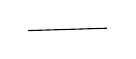
\begin{tikzpicture}[x=1mm,y=1mm]\draw (0,0)--(10,.3);\end{tikzpicture}}

\deleted{\unsure{Les}} \uline{\unsure{Correspondances} entre \inserted{disjoncteurs et entre} \unsure{Spatios|Spotos}.} $\deleted{\unsure{\Sigma}}$

\deleted{\unsure{Les|des}} \uline{Analogie} Soient $E,E'$ deux ensembles, \deleted{\unsure{i.e.}} ou encore disjoncteurs triviaux. Une ``corr'' (ou ``relation'' \inserted{$R$}) entre $E,E'$ peut \unsure{être|etre} \unsure{interprétée} comme une application
\[
\unsure{\alpha|\varphi}:E\unsure{{-}|\longrightarrow}\unsure{\mathscr{P}|\mathcal{P}|\mathfrak{P}}(E')
\qquad(x\unsure{\longmapsto|{\mid}{-}}R(x))
\]
